\documentclass[11pt]{article}

% ---------- Page & Font ----------
\usepackage[margin=2.5cm]{geometry}
\usepackage[utf8]{inputenc}
\usepackage[T1]{fontenc}
\usepackage{lmodern}
\usepackage{microtype}

% ---------- Math & Units ----------
\usepackage{amsmath, amssymb}
\usepackage{siunitx}
\sisetup{per-mode=symbol}

% ---------- Figures & Tables ----------
\usepackage{graphicx}
\usepackage{caption}
\usepackage{subcaption}
\usepackage{float}
\usepackage{booktabs}
\usepackage{array}
\usepackage[table]{xcolor}

% ---------- Code Listings (C, C++, Rust) ----------
\usepackage{listings}
\usepackage{xcolor}

\definecolor{codebg}{RGB}{245,245,245}
\definecolor{codegray}{RGB}{110,110,110}
\definecolor{codeblue}{RGB}{0,80,180}
\definecolor{codegreen}{RGB}{0,120,0}
\definecolor{codered}{RGB}{170,0,0}

\lstdefinelanguage{Rust}{
  keywords={fn, let, mut, pub, struct, enum, impl, trait, for, while, loop, if, else, match, return, use, mod, crate, self, Self, in, as, ref, move, unsafe, dyn, where, const, static, type},
  keywordstyle=\color{codeblue}\bfseries,
  ndkeywords={u8,u16,u32,u64,usize,i8,i16,i32,i64,isize,f32,f64,bool,char,str,String,Vec,Option,Result,Box},
  ndkeywordstyle=\color{codegreen},
  identifierstyle=\color{black},
  sensitive=true,
  comment=[l]{//},
  morecomment=[s]{/*}{*/},
  commentstyle=\color{codegray}\itshape,
  stringstyle=\color{codered},
  morestring=[b]",
}

\lstset{
  backgroundcolor=\color{codebg},
  basicstyle=\ttfamily\footnotesize,
  breaklines=true,
  breakatwhitespace=false,
  frame=single,
  rulecolor=\color{black!20},
  numbers=left,
  numberstyle=\tiny\color{codegray},
  numbersep=8pt,
  showstringspaces=false,
  tabsize=2,
  captionpos=b,
  keywordstyle=\color{codeblue}\bfseries,
  commentstyle=\color{codegray}\itshape,
  stringstyle=\color{codered},
}

% Convenience environments per language
\lstnewenvironment{ccode}[1][]{\lstset{language=C,#1}}{}
\lstnewenvironment{cppcode}[1][]{\lstset{language=C++,#1}}{}
\lstnewenvironment{rustcode}[1][]{\lstset{language=Rust,#1}}{}

% ---------- Misc ----------
\usepackage{hyperref}
\hypersetup{colorlinks=true, linkcolor=blue, citecolor=blue, urlcolor=blue}
\usepackage{enumitem}
\usepackage{xurl}

% ---------- Custom colored boxes for special sections ----------
\usepackage[most]{tcolorbox}

\newtcolorbox{hypothesisbox}{
  colback=blue!4, colframe=blue!50!black, title=Pre-Experiment Hypothesis,
  fonttitle=\bfseries, breakable
}
\newtcolorbox{failurebox}{
  colback=red!4, colframe=red!50!black, title=Negative / Failure Case,
  fonttitle=\bfseries, breakable
}
\newtcolorbox{anomalybox}{
  colback=yellow!8, colframe=orange!70!black, title=Honest Anomalies,
  fonttitle=\bfseries, breakable
}

% ---------- Title Info ----------
\title{\textbf{ECSE-6320 Advanced Computer Systems \\ Project 2 Report}}
\author{Cooper Werner \\\small Rensselaer Polytechnic Institute \\ \small wernec6@rpi.edu}
\date{\today}

\begin{document}

\maketitle

\tableofcontents
\newpage

% =====================================================
\section{Introduction}
% Context, motivation, system under test, and objective of this experiment.

% =====================================================

The goal of this project is to analyze how the memory hierarchy impacts memory performance as the working set size,
data stride, access pattern, read-write ratio, and access intensity, changes.

To do this I will use 4 different computational kernels:

\begin{enumerate}
	\item Array Reduction, Summing all values of an array: 100\% read.
	\item Memset, setting all values in an array to one value: 100\% write.
	\item Vector-Vector Multiply, element-wise multiplication of two vectors: 66\% read / 33\% write.
	\item Scalar-Vector Multiply, element-wise multiplication with a scalar: 50 \% read / 50\% write.
\end{enumerate}

To change the other experimental variables, I have a main kernel runner that can control the working set size, the
stride of the data, run with random access patterns, number of threads accessing the data. To be able to control the
page size, I will be running this code in a Linux VM where I can set the memory page size to either 4KiB or 2MiB.

I also make use of Intel Memory Latency Checker (MLC) to determine latency and bandwidth at different read write
ratios, access patterns, and memory queue depths.

\section{Pre-Experiment Hypotheses}

\begin{hypothesisbox}
	\textbf{Hypothesis:} \\
	% State the falsifiable prediction before running anything.

	As the MLC injection delay decreases (and thus the memory queue depth increases) bandwidth will increase as the memory
	will make better use of the queue. However, since the queue is being fully utilized, the latency of any one specific
	data transfer request will be higher as it needs to wait in the queue to be fulfilled.

	\textbf{Reasoning:} \\
	% Why do you expect this outcome? Reference architecture, prior results, theory.

	Little's law defines $L = \lambda R$, decreasing the injection delay, will increase the number of outstanding requests,
	$L$. By Little's law, the response time must increase. However, since there are more requests in flight, more data will
	be transferred as the bus will stay more active.

	\textbf{Predicted quantitative outcome:} \\
	\begin{center}
		\captionof{table}{Latency and Bandwidth Figures vs Injection Delay}
		\label{tab:hypothesis-huge-pages}
		\begin{tabular}{lcc}
			\toprule
			\textbf{Injection Delay (ns)} & \textbf{Single Request Latency (ns)} & \textbf{Total Bandwidth} \\
			\midrule
			20,000                        & $50$ ns                              & $20$ GB/s                \\
			15,000                        & $75$ ns                              & $30$ GB/s                \\
			10,000                        & $100$ ns                             & $40$ GB/s                \\
			5,000                         & $200$ ns                             & $50$ GB/s                \\
			2,500                         & $400$ ns                             & $55$ GB/s                \\
			0                             & $800$ ns                             & $60$ GB/s                \\
			\bottomrule
		\end{tabular}
	\end{center}
\end{hypothesisbox}

\begin{hypothesisbox}
	\textbf{Hypothesis:} \\
	% State the falsifiable prediction before running anything.

	The random access pattern will have the most TLB and Cache misses of all of the stride / access patterns since it will
	be constantly jumping around the address space to fetch data for the computations.

	\textbf{Reasoning:} \\
	% Why do you expect this outcome? Reference architecture, prior results, theory.

	The random access pattern will be jumping around the memory space to figure out which memory elements need to be
	fetched. This will mean an elevated number of cache misses for data that doesn't fit in the cache, and an elevated
	number of TLB misses since cache lines will constantly have to be moved into and out of memory.

	\textbf{Predicted quantitative outcome:} \\
	% e.g., "Expect L2 miss rate to decrease by \SI{15}{\percent} \pm \SI{3}{\percent}"
	\begin{center}
		\captionof{table}{Predicted TLB Walk and Cache Miss Rates for different access patterns. }
		\label{tab:hypothesis-simd}
		\begin{tabular}{lcc}
			\toprule
			\textbf{Access Pattern} & \textbf{Cache Miss Rate} & \textbf{TLB Walk Rate} \\
			\midrule
			Stride 0B               & 10\%                     & 5\%                    \\
			Stride 16B              & 20\%                     & 6\%                    \\
			Stride 32B              & 30\%                     & 7\%                    \\
			Stride 64B              & 40\%                     & 8\%                    \\
			Stride 128B             & 50\%                     & 9\%                    \\
			Random                  & 55\%                     & 10\%                   \\
			\bottomrule
		\end{tabular}
	\end{center}
\end{hypothesisbox}

% =====================================================

% =====================================================
\section{Measurement Discipline}
% Describe methodology: isolation (core pinning, turbo/frequency scaling disabled, etc.),
% number of trials, warm-up runs, statistical treatment (mean/median/stdev/CI),
% timer resolution, environmental controls.

To gather data for this project I used two tools. The first tool I used was Intel's Memory Latency Checker (MLC), this
tool varies RAM injection delay, read write ratios, and stride sizes to measure memory bandwidth and latency for
different queue depths. The second tool I used was a series of C programs that ran simple computational kernels to
Benchmark cache and TLB misses for different access patterns, read/write mixes, and working set sizes.

\subsection{Experimental Setup}
\begin{itemize}[leftmargin=1.5em]
	\item \textbf{Hardware:} CPU: x86\_64 AMD Ryzen AI 7 350 w/ Radeon 860M, Memory: 32GB LPDDR5 @ 5600MT/s
	\item \textbf{OS / Kernel:} Pop\_OS! 24.04 Running Linux 7.0.11-76070011-generic page size fixed at 4096B per page.
	\item \textbf{Compiler \& Flags:} GCC 16.2.0, Flags: -O3
	\item \textbf{Trials per condition:} 10 trials per condition
	\item \textbf{Timer / Instrumentation:} clock\_gettime(CLOCK\_MONOTONIC), Linux perf header + hardware event counters for measuring TLB and memory events, Intel Memory Latency Checker
	\item \textbf{Intel MLC Version: } 3.2.1
\end{itemize}

The mean result from each trial is then plotted on each chart and is reported. For the working set sweep, the median
and minimum times are reported to remove any noise from the kernel computations.

\subsection*{Performance Measure Definitions}

This specific AMD CPU has some strange quirks when it comes to interfacing with performance counters that complicate
the definitions for the specific performance measures used.

\begin{enumerate}
	\item LLC Miss Rate: L3 Cache Miss Rate, the AMD performance counters call L3 Cache ``LLC'' Cache.
	\item TLB Miss Rate: \# of Page Walks / \# of Loads, this CPU has a two level TLB, this means that there are multiple
	      definitions for TLB Miss rate: L1 TLB misses where L2 TLB hits, L2 TLB Misses, or all page walks since the CPU will
	      sometime prefetch addresses for the L2 TLB. To quantify this into one number I chose \# of Page Walks / \# of Loads as
	      it best represents the way we think about a TLB miss.
\end{enumerate}

\section{Results}

\begin{figure}[H]
	\centering
	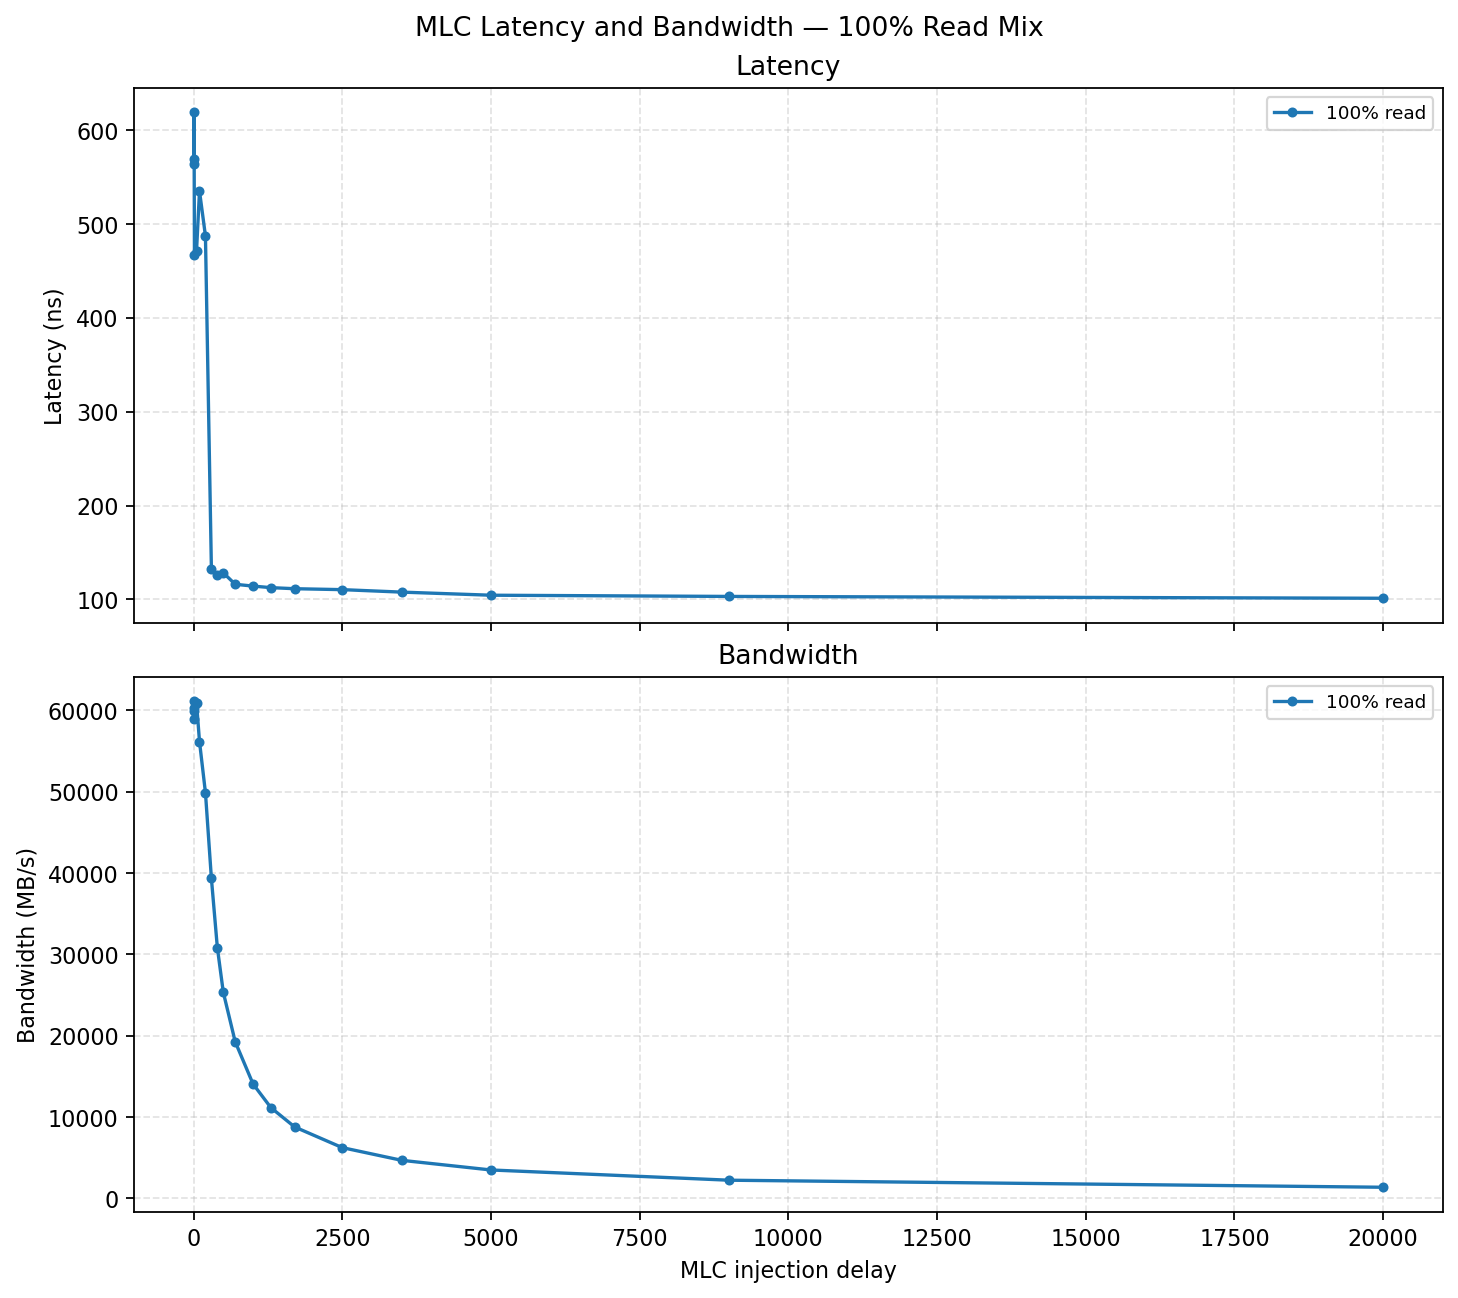
\includegraphics[width=0.85\textwidth]{../analysis/mlc_100_read_latency_bandwidth.png}
	\caption{Plot of bandwidth and latency vs injection delay. Lower injection delay creates a longer queue. The longer queue means that the DRAM bus is more fully
		utilized but that the latency of each individual request increases as the requests must wait in the queue before being fulfilled. Latency and Bandwidth start
		tradeoff at an injection delay of 300ns. With an injection delay less than 300ns the queue becomes full enough to start maximizing bandwidth at the cost of
		request latency. Above 300ns, the queue is empty enough where latency is more dependent on the access speed of the DRAM itself. This follows the expectation of Little's law
		albeit, less linearly than the equation $L = \lambda R$ may suggest.}
	\label{fig:100read-bandwidth-latency}
\end{figure}

\begin{table}[H]
	\centering
	\caption{Zero Queue Baseline Latency Across the Memory Hierarchy}
	\label{tab:zero-queue-baseline}
	\begin{tabular}{@{}lccc@{}}
		\toprule
		Memory Level & Latency (ns) & CPU Clocks & CPU Frequency (MHz) \\
		\midrule
		L1           & 0.8          & 1.6        & 2000                \\
		L2           & 2.8          & 5.5        & 2000                \\
		LLC          & 11.3         & 22.6       & 2000                \\
		DRAM         & 136.1        & 271.7      & 2000                \\
		\bottomrule
	\end{tabular}
\end{table}

\begin{figure}[H]
	\centering
	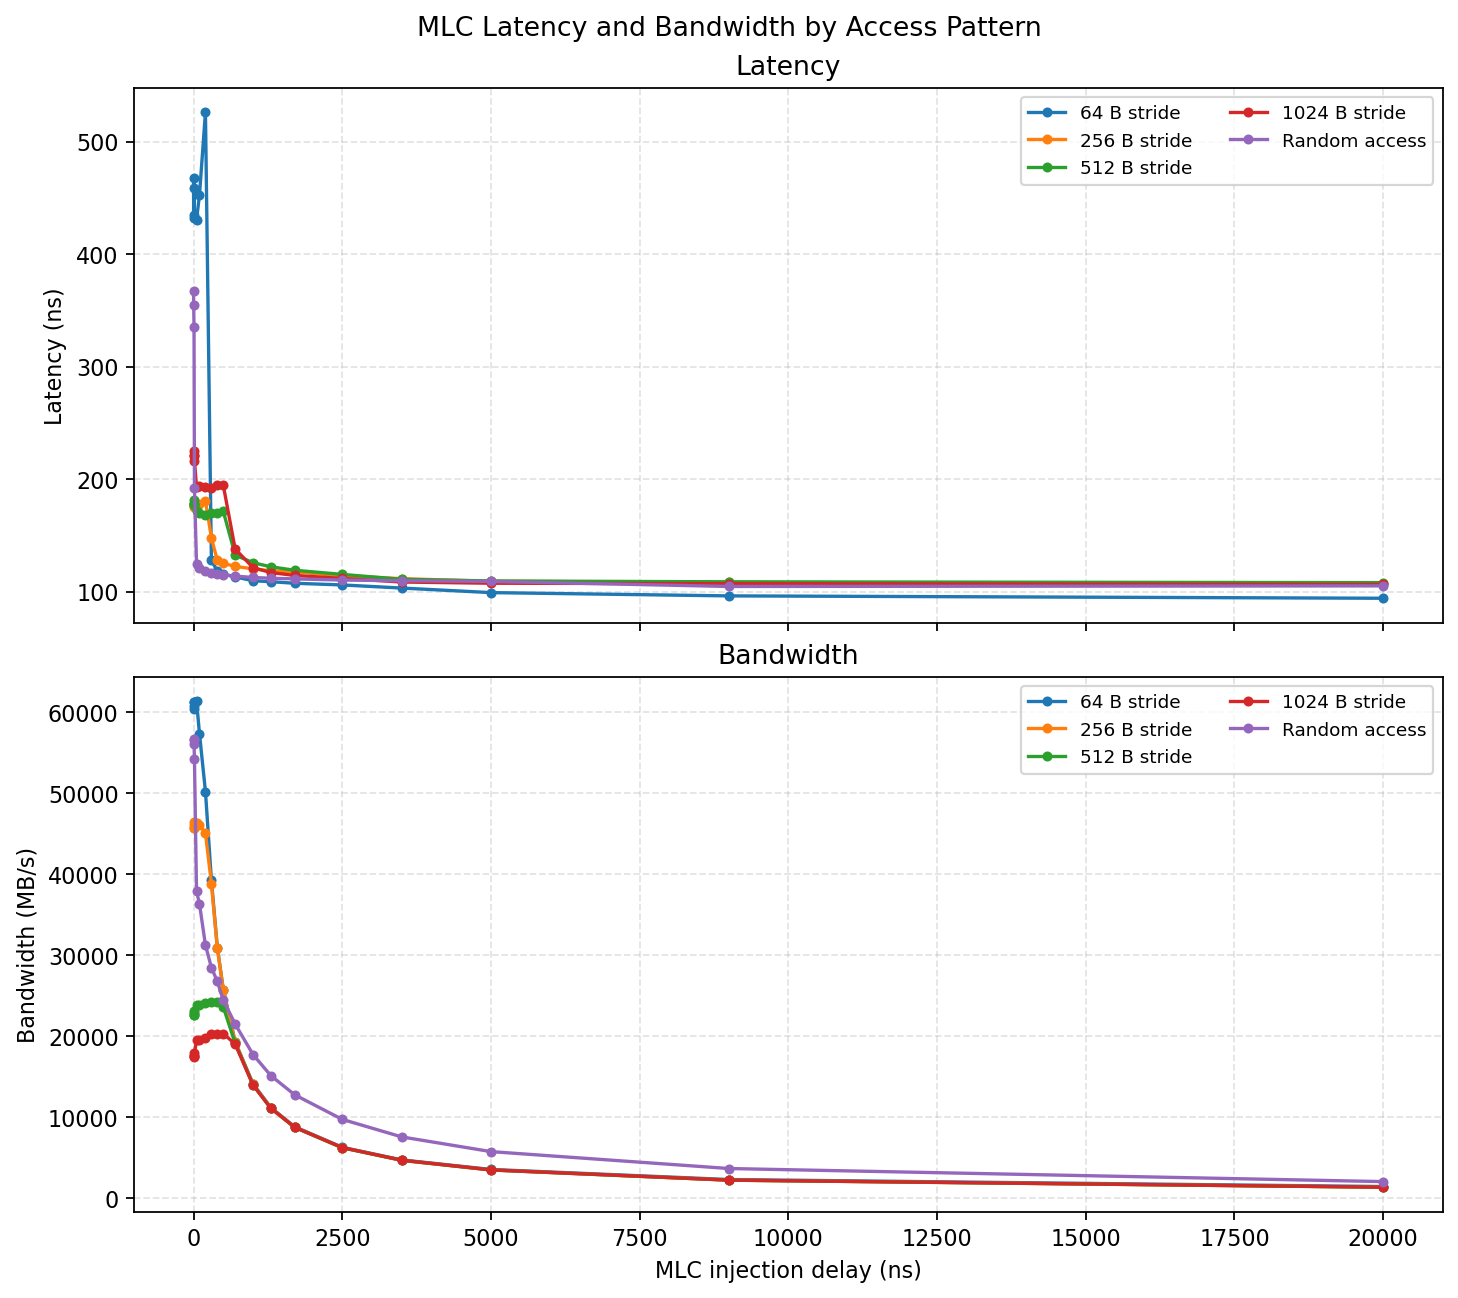
\includegraphics[width=0.85\textwidth]{../analysis/mlc_access_pattern_latency_bandwidth.png}
	\caption{Plot of bandwidth and latency vs injection delay with different stride/access patterns. Little's law still shows a tradeoff between
		latency and bandwidth at an injection delay around 300ns. However, when the stride reached 512 bytes, the maximum bandwidth dropped significantly,
		so did the maximum latency. }
	\label{fig:latency-bandwidth-access-pattern}
\end{figure}

\begin{figure}[H]
	\centering
	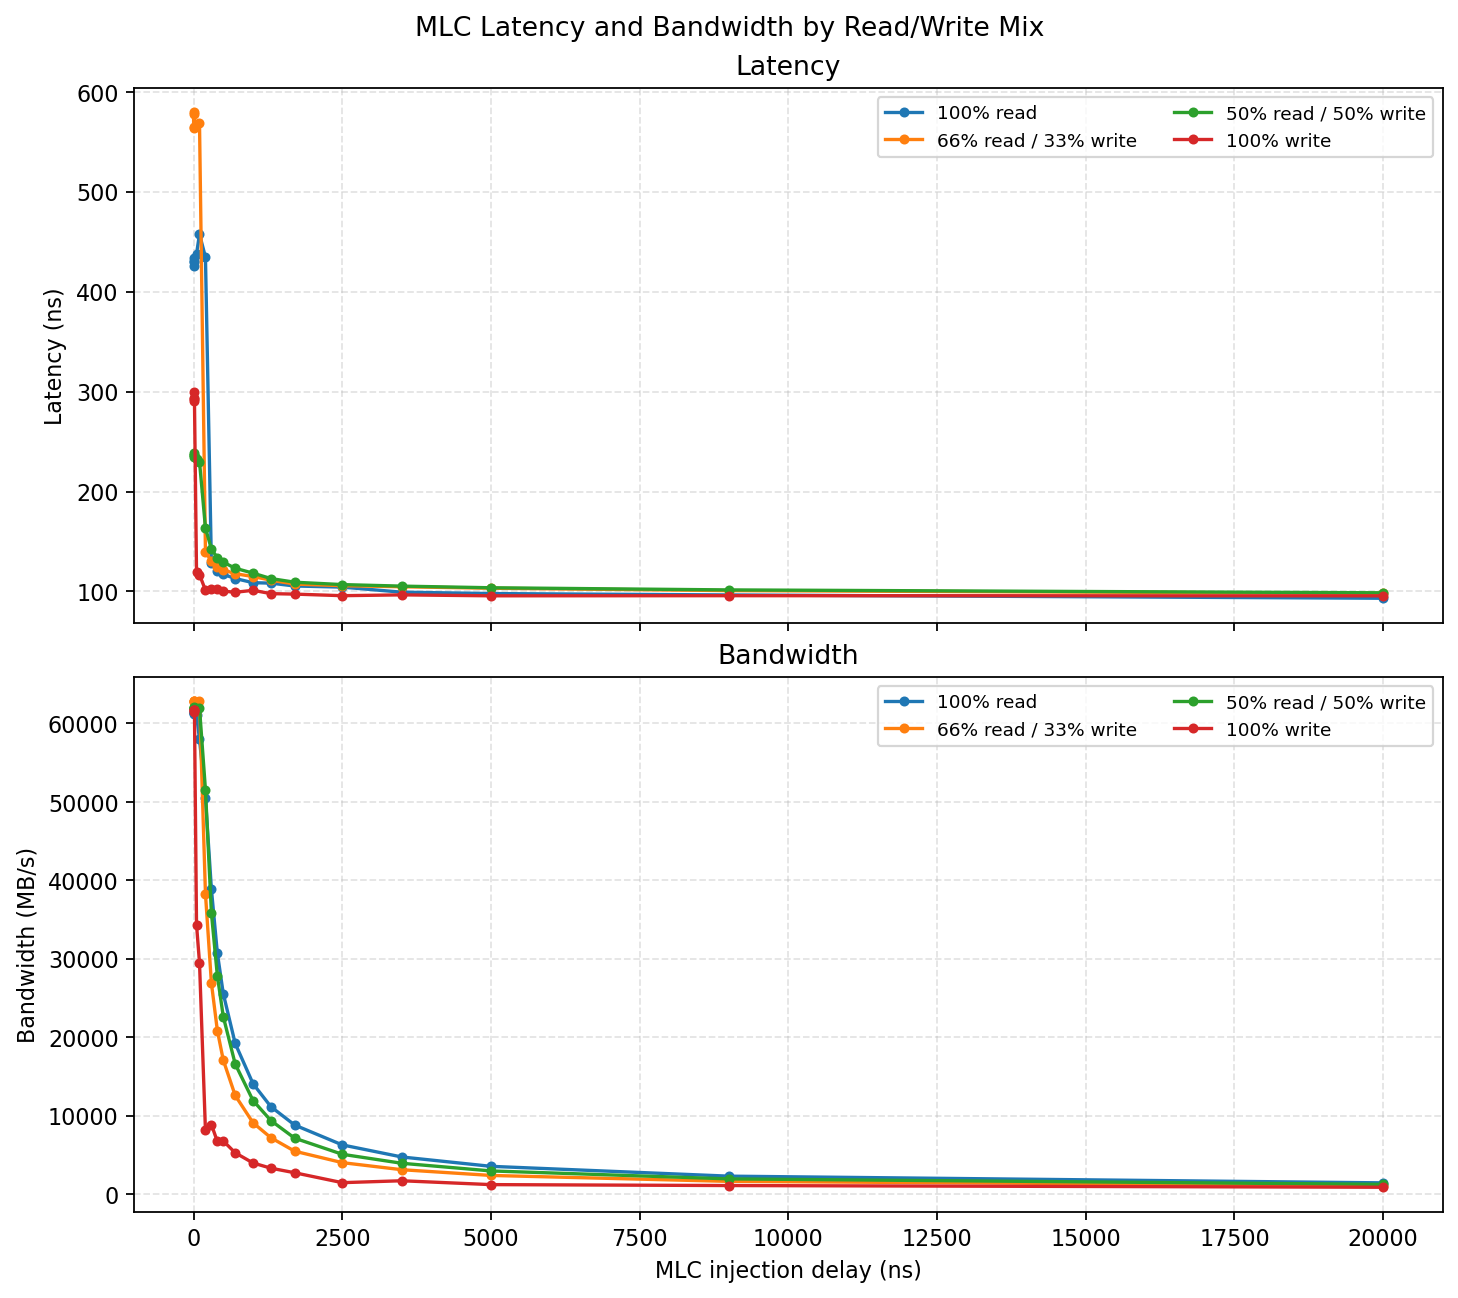
\includegraphics[width=0.85\textwidth]{../analysis/mlc_read_write_mix_latency_bandwidth.png}
	\caption{Plot of bandwidth and latency vs injection delay for different read-write mixes. The specific mix doesn't significantly change the point at which
		Little's Law starts to trade latency for bandwidth. The interesting observation from this is that the more write heavy mixes have significantly lower
		latency despite still reaching the same peak bandwidth.}
	\label{fig:latency-bandwidth-read-write-mix}
\end{figure}

\begin{figure}[H]
	\centering
	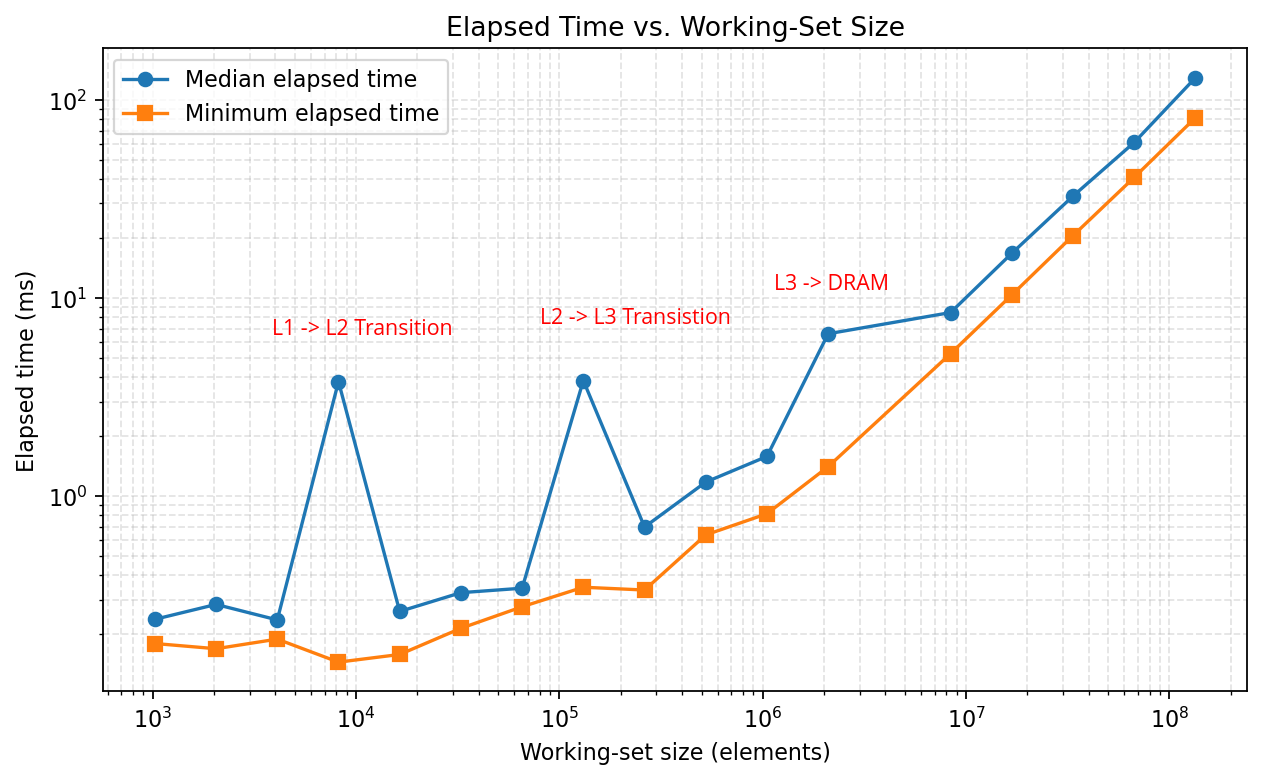
\includegraphics[width=0.85\textwidth]{../analysis/working_set_elapsed_time.png}
	\caption{Plot of time to compute kernels as working set size changes. The transition times for each layer are annotated on the graph. There is a
		spike in median execution times when the data transitions regions in the memory. The minimum execution time also shows these transitions as the slope
		of the plot changes as the location of the data changes. }
	\label{fig:working-set-elapsed-time}
\end{figure}

\begin{figure}[H]
	\centering
	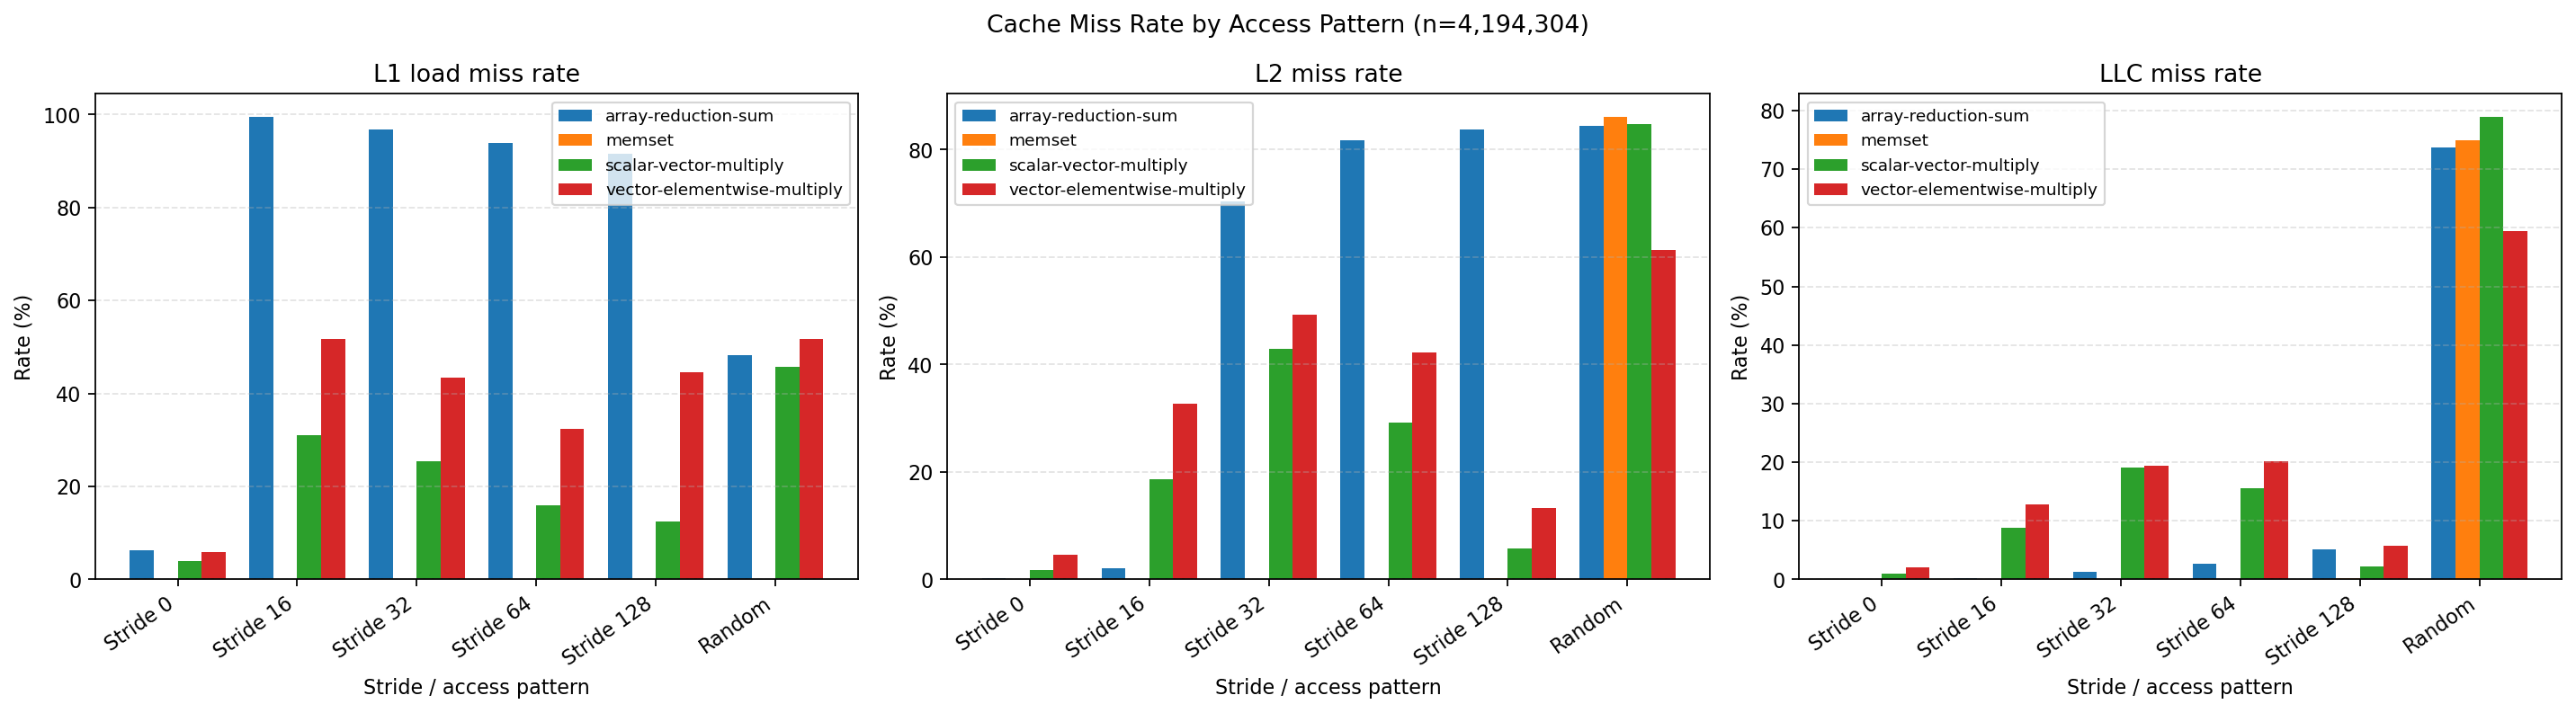
\includegraphics[width=0.85\textwidth]{../analysis/cache_miss_rate_by_access_pattern.png}
	\caption{Bar Chart showing the cache miss rates for each cache level. Cache miss rates are captured using the CPU's performance counters.
		L1 cache miss rates for memset are not captured as memset only writes to memory, and on this CPU, memory writes don't write to L1 cache.
		The random access pattern consistently has one of the highest cache miss rates with the exception of the L1 cache on array reduction. This makes
		sense as all the data is tightly packed, just randomly accessed instead of being spread out like it is with strided data patterns.}
	\label{fig:cache-miss-access-pattern}
\end{figure}

\begin{figure}[H]
	\centering
	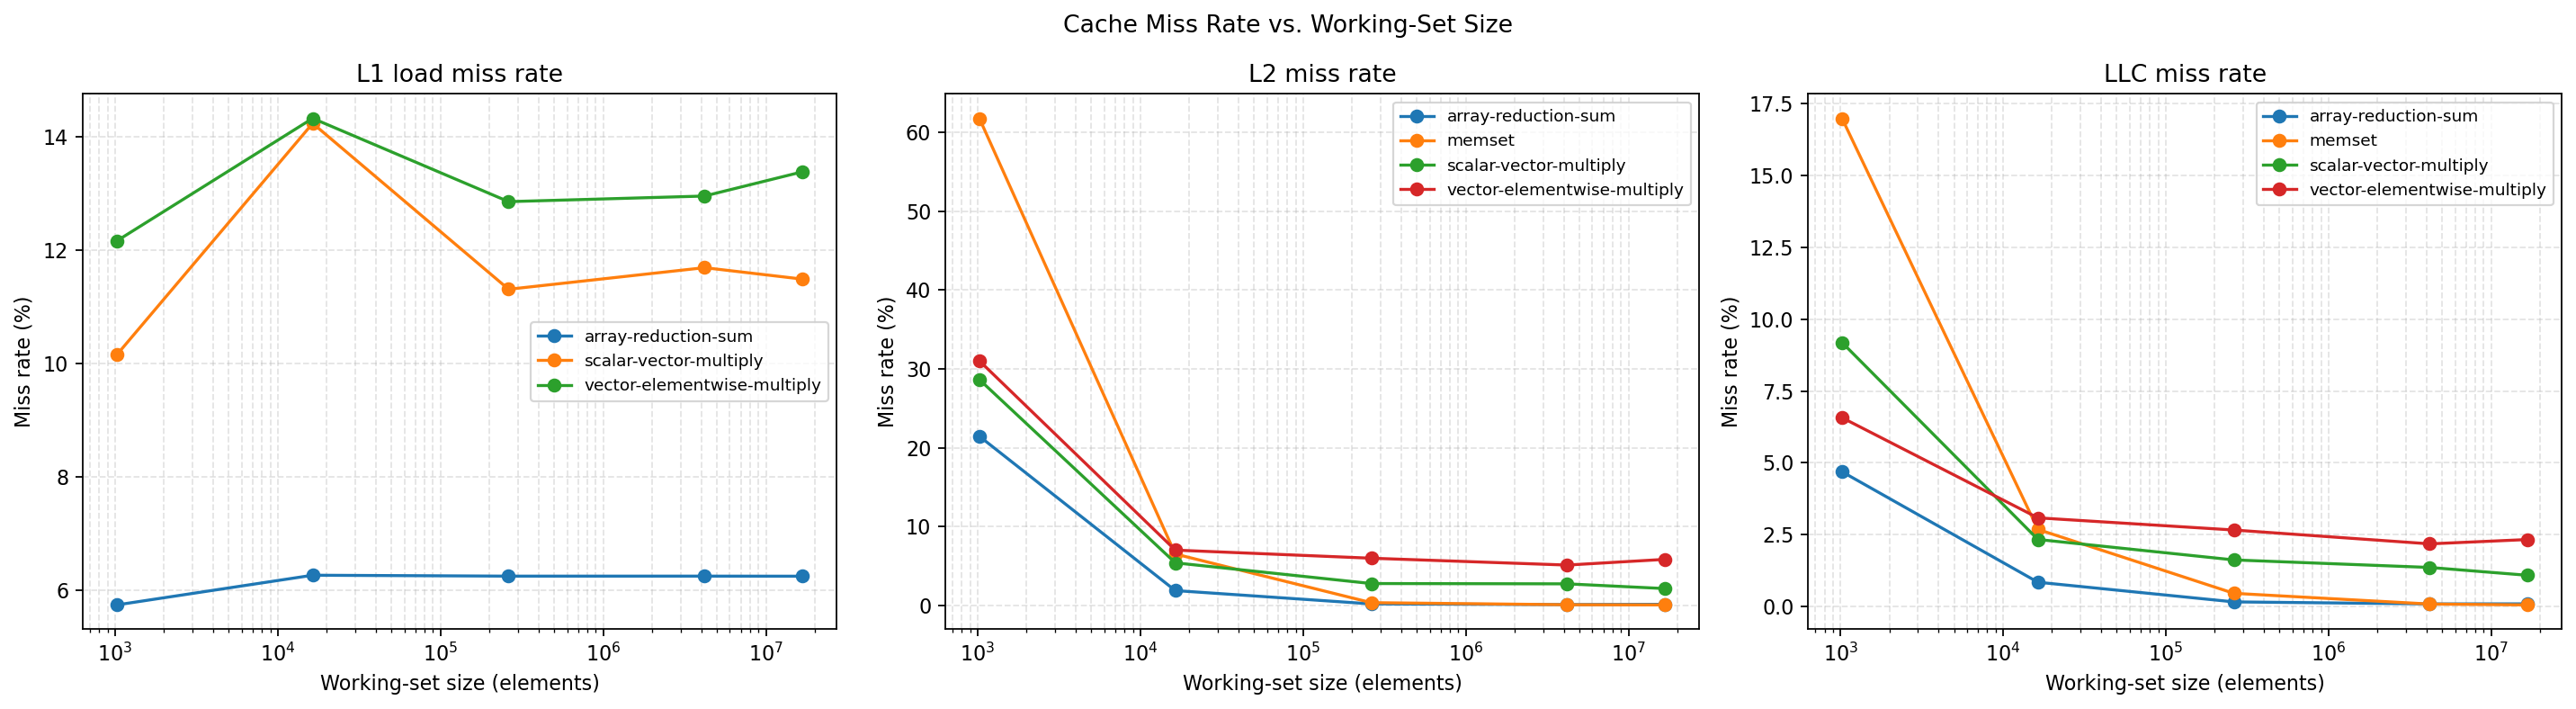
\includegraphics[width=0.85\textwidth]{../analysis/cache_miss_rate_vs_working_set_size.png}
	\caption{Plot of cache miss rate as working set size increases. L1 cache for memset is not reported as memory writes do not write to L1 cache.
		L1 cache misses stay mostly even as working size increases because the cache is small enough where after a certain point, L1 misses are inevitable. L2 and L3 cache miss rate
		decrease as working set size increases, this is likely due to the cache being able to fill itself with valid data once the working set reaches a proper size, reducing the
		number of misses due to not having the data loaded into cache in the first place.}
	\label{fig:cache-miss-working-set}
\end{figure}

\begin{figure}[H]
	\centering
	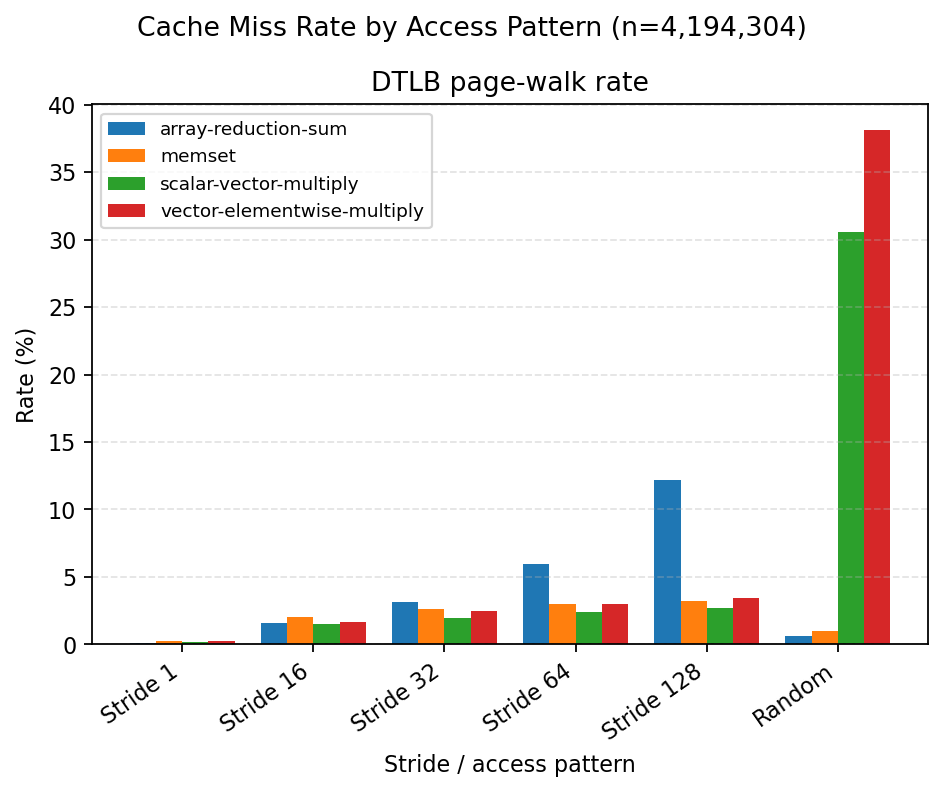
\includegraphics[width=0.85\textwidth]{../analysis/page_walk_rate_by_access_pattern.png}
	\caption{Bar chart showing the page walk rate for each access pattern and kernel.
		The random access pattern has a significantly higher page walk rate for the vector-scalar and vector-vector multiplication kernels. The
		page walk rate for the memset and vector reduction kernels is significantly smaller than I would have expected. The walk rate is larger than
		a stride of 1, but not much larger. It would be interesting to investigate this more. Perhaps this may be due to the metric I define as page
		walk rate as number of page walks / number of loads.}
	\label{fig:page-walk-rate-access-pattern}
\end{figure}

\begin{figure}[H]
	\centering
	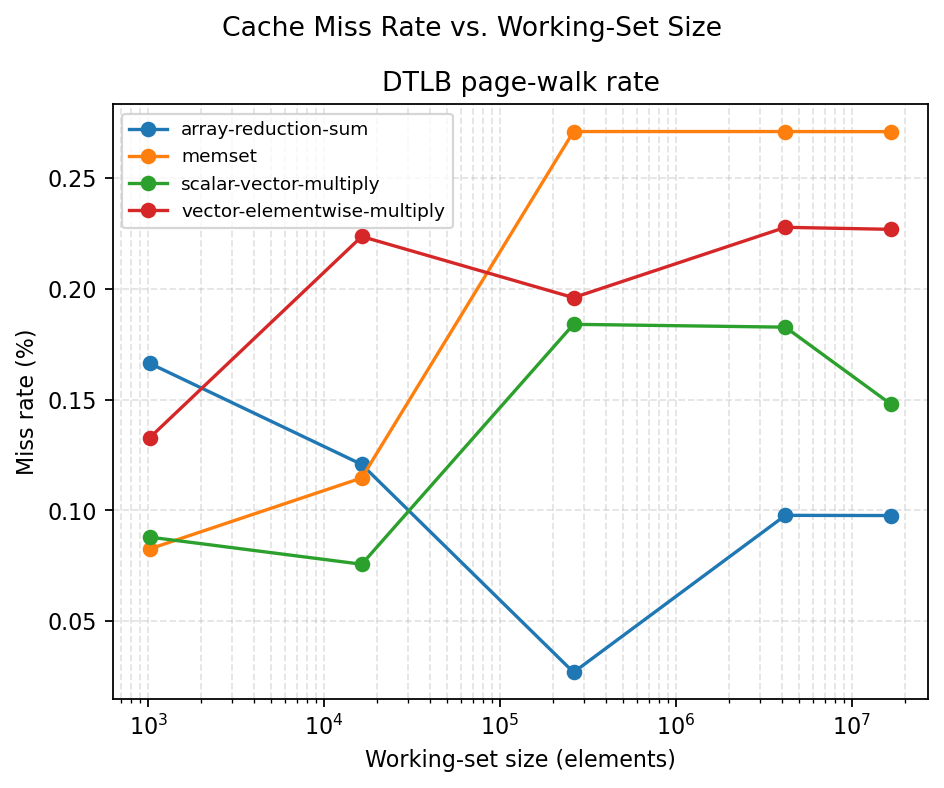
\includegraphics[width=0.85\textwidth]{../analysis/page_walk_rate_vs_working_set_size.png}
	\caption{Plot of page walk rate as working set size changes. Most kernels show an increase in the page walk rate as working set size increases.
		The vector reduction kernel doesn't display this trend however, the page walk rate stays flat or even decreases as the working set size increases.
		I am not exactly why this is. More exploration into this may be interesting.}
	\label{fig:page-walk-rate-working-set-size}
\end{figure}

% =====================================================
\section{Negative / Failure Case}

\begin{failurebox}
	\textbf{What failed:} \\
	% Configuration, workload, or condition that did NOT behave as expected or hypothesized.
	My method for measuring TLB page walks likely is not the best way to measure TLB misses. Since this computer has
	multiple TLB levels and a page table walk can be triggered to fill up the L2 TLB instead of just when a single TLB
	entry is missing, profiling TLB misses becomes much more nuanced than I tested in this project.

	\textbf{Evidence:} \\
	% Data, logs, or figure reference showing the failure.

	I think this is best shown in Figures \ref{fig:page-walk-rate-access-pattern} and
	\ref{fig:page-walk-rate-working-set-size} where we see those page walk rate anomalies with array-reduction and memset.

	\textbf{Root cause (if known):} \\

	My current measurement reports the number of page walks divided by the total number of load operations. This likely
	skews the rate for kernels where there are very few loads or many loads. THis would correlate with the array-reduction
	and memset operations as they are both 100\% read or 100\% write kernels.

\end{failurebox}

% =====================================================
\section{Discussion}
% Tie hypothesis, validation, results, and anomalies together. Was the hypothesis supported,
% refuted, or inconclusive? What would you do differently next time?

% =====================================================

I think that my hypotheses had the right idea, but I underestimated the rate at which Little's law would impact
bandwidth vs latency and the cache miss rate for the different access patterns. I thought that because of the linearity
in the equation for Little's law, $L = \lambda R$ I figured that the tradeoff between latency and bandwidth would be
more linear. The tradeoff was not linear, it was instead very sudden and only happened when the queue got close to its
maximum depth.

For the cache miss rate hypothesis, the trend I predicted was correct, and the magnitude I predicted was mostly
correct. Although, this comes with the notable exception from the array reduction kernel that had a significantly
higher cache miss rate. I think this is due to the fact that the kernel was only reading and didn't have to wait on
writes to complete. I am not certain of this though.

I think the thing that surprised me the most was the latency figures for L1, L2, L3, and DRAM latency at idle and 0
queue depth. I didn't realize that even L3 cache was up to 10x faster than a DRAM fetch.

\section{Conclusion}

Optimal usage of DRAM requires careful attention to DRAM queue depth, data layout, and cache utilization. Programs that
fail to properly utilize cache, keep data contiguous in memory, and fail to manage DRAM accesses can suffer from
significantly larger DRAM latency, decreased bandwidth, or an increased cache miss rate. Considering how much faster
even L3 cache is than DRAM, its important that programmers think about how data structures can best utilize the memory
hierarchy.

% =====================================================
\appendix

\section{AI Usage}

AI helped me write the code required for the experiment, it helped develop scripts for running all the required
experiments, assisted in developing python code to create plots and figures. Lastly, I utilized AI in developing the
experimental design and troubleshooting anomalies in the data.

\begin{enumerate}
	\item Helped me debug TLB counting issues: https://claude.ai/share/260b7e8a-715a-4fc9-b35f-1a8da1b12fc6
	\item Helped me debug an issue with Intel MLC: https://claude.ai/share/afe27cd9-13a4-40b0-9c47-f0005b25f7b5
\end{enumerate}

I also made extensive use of OpenCode (an open source coding agent) to develop scripts, experiment code, and plotting
code. I reveiewed all output for correctness and accuracy. Making minor fixes where applicable. Transcripts for the
OpenCode sessions are available in \texttt{./OpenCode}

\section{Additional Data / Raw Logs}
% Optional: full result dumps, extra plots, raw perf output, etc.
The raw data is available in the \texttt{./results} directory. Images of all the plots and the plotting code is
available in the \texttt{./analysis} directory.

\end{document}